\chapter{Common Distributions}\label{ch:common-distributions}

\chapterinfo{STAT2003, STAT1301}{\cref{ch:probability-spaces,ch:random-variables,ch:expectation-moments,ch:generating-functions}.}

% Sources: STAT2003 handwritten notes (pp. 14-25); STAT2003 course notes, Sections 2.5-2.6;
% STAT1301 course notes (2026), Sections 2.1-2.5 and Table 2.1.

This chapter lists the most important discrete and continuous distributions, with their main properties. The pmf or pdf of each depends on one or more \emph{parameters}, fixed values that determine the shape of the distribution, so each is really a \emph{family} of distributions. Although statistics uses a relatively small collection of families, choosing the parameters gives an infinite number of distributions.

% ==========================================================================
\section{Bernoulli trials}\label{sec:bernoulli-trials}
% ==========================================================================

A \emph{Bernoulli trial} is a random experiment with only two possible outcomes, usually labelled ``success'' (1) and ``failure'' (0). Examples are a single coin toss (1 for heads, 0 for tails), or selecting a person at random from a population and asking whether they approve of the prime minister.

\begin{definition}[i.i.d.]\label{def:iid}
Random variables (or trials) are \emph{i.i.d.} if they are \emph{independent and identically distributed}.
\end{definition}

Most of the important discrete distributions are associated with a sequence of i.i.d.\ Bernoulli trials. They are all induced by the same probability space: $\Omega$ is the set of sequences of coin flips, such as $HHH\ldots$ or $HTH\ldots$, and if $A_i$ is the event that flip $i$ is a success (1), then $\Prob(A_i) = p$ and
\[
  \Prob(A_{i_1} \cap A_{i_2} \cap \cdots \cap A_{i_k}) = \Prob(A_{i_1}) \cdots \Prob(A_{i_k})
\]
for any distinct indices $i_1, \ldots, i_k$ (\cref{sec:coin-tossing-models}). The distributions differ in what they count:
\begin{itemize}
  \item Bernoulli: the outcome of a single trial (values 0 and 1)
  \item binomial: the number of successes in $n$ trials (values $0, 1, \ldots, n$)
  \item geometric: the number of trials until the first success (values $1, 2, \ldots$)
  \item negative binomial: the number of trials until the $k$th success (values $k, k+1, \ldots$)
\end{itemize}

\begin{figure}[H]
\centering
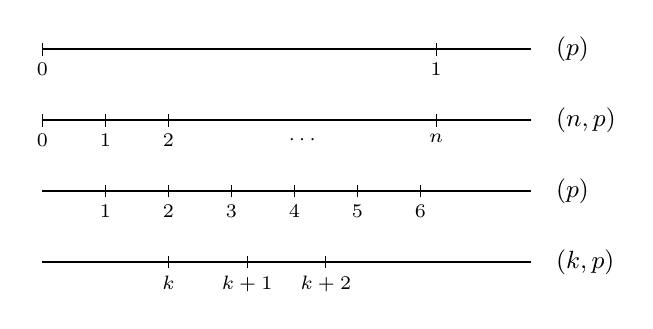
\begin{tikzpicture}
  \foreach \y/\lab/\m in {0/{$\Bern(p)$}/1, -0.9/{$\Bin(n,p)$}/2, -1.8/{$\Geom(p)$}/3, -2.7/{$\NegBin(k,p)$}/4} {
    \draw[thick] (0,\y) -- (6.2,\y);
    \node[anchor=west, font=\small] at (6.4,\y) {\lab};
  }
  \foreach \x/\l in {0/0, 5/1} { \draw (\x,-0.08) -- (\x,0.08); \node[font=\scriptsize, below] at (\x,-0.05) {\l}; }
  \foreach \x/\l in {0/0, 0.8/1, 1.6/2, 5/n} { \draw (\x,-0.98) -- (\x,-0.82); \node[font=\scriptsize, below] at (\x,-0.95) {$\l$}; }
  \node[font=\scriptsize] at (3.3,-1.15) {$\cdots$};
  \foreach \x/\l in {0.8/1, 1.6/2, 2.4/3, 3.2/4, 4.0/5, 4.8/6} { \draw (\x,-1.88) -- (\x,-1.72); \node[font=\scriptsize, below] at (\x,-1.85) {\l}; }
  \foreach \x/\l in {1.6/k, 2.6/{k+1}, 3.6/{k+2}} { \draw (\x,-2.78) -- (\x,-2.62); \node[font=\scriptsize, below] at (\x,-2.75) {$\l$}; }
  \node at (6.6,-2.7) {};
\end{tikzpicture}
\caption{Possible values of the Bernoulli, binomial, geometric and negative binomial random variables, all defined from the same sequence of i.i.d.\ Bernoulli trials.}
\label{fig:bernoulli-family-supports}
\end{figure}


% ==========================================================================
\section{Discrete distributions}\label{sec:discrete-families}
% ==========================================================================

\subsection{Bernoulli distribution}\label{sec:bernoulli}

\begin{definition}[Bernoulli distribution]\label{def:bernoulli}
$X$ has a \emph{Bernoulli distribution} with success probability $p$ if $X$ can only take the values 0 and 1, with
\[
  \Prob(X = 1) = p = 1 - \Prob(X = 0).
\]
We write $X \sim \Bern(p)$.
\end{definition}

Despite its simplicity, this is one of the most important distributions in probability. It models, for example, a single coin toss.

\begin{figure}[H]
\centering
\begin{tikzpicture}
\begin{axis}[pmfplot, width=0.45\textwidth, height=4cm, xmin=-0.5, xmax=1.5, ymax=0.7, xtick={0,1}, xlabel={$x$}, ylabel={$f(x)$}]
  \addplot coordinates {(0,0.4) (1,0.6)};
\end{axis}
\end{tikzpicture}
\caption{The pmf of the Bernoulli distribution with $p = 0.6$.}
\label{fig:bernoulli-pmf}
\end{figure}


\begin{theorem}[Properties of the Bernoulli distribution]\label{thm:bernoulli-properties}
Let $X \sim \Bern(p)$. Then
\begin{enumerate}
  \item $\E X = p$
  \item $\Var(X) = p(1-p)$
  \item the PGF is $G(z) = 1 - p + zp$
\end{enumerate}
\end{theorem}

\begin{proof}\leavevmode
\begin{enumerate}[leftmargin=*]
  \item[1.] $\E X = 0 \cdot \Prob(X = 0) + 1 \cdot \Prob(X = 1) = 0 \cdot (1-p) + 1 \cdot p = p$.
  \item[2.] Since $X^2 = X$, $\Var(X) = \E X^2 - (\E X)^2 = \E X - (\E X)^2 = p - p^2 = p(1-p)$.
  \item[3.] $G(z) = z^0 (1-p) + z^1 p = 1 - p + zp$. \qedhere
\end{enumerate}
\end{proof}

\subsection{Binomial distribution}\label{sec:binomial}

Flip a fair coin 100 times and let $X$ be the number of successes (heads). $X$ can take the values $0, 1, \ldots, 100$. There are $2^{100}$ equally likely sequences of tosses, and $\binom{100}{x}$ of them have exactly $x$ ones, since we must choose $x$ positions for the ones out of 100. So
\[
  \Prob(X = x) = \frac{\binom{100}{x}}{2^{100}}, \qquad x = 0, 1, \ldots, 100.
\]
For example, $\Prob(X \ge 60) = \sum_{x=60}^{100} \binom{100}{x} / 2^{100}$, which can be evaluated in R:
\begin{rcode}
sum(choose(100, 60:100)) / 2^100    # 0.02844397
\end{rcode}

More generally, if the probability of heads is $p$, the outcomes are no longer equally likely. By the product rule (\cref{thm:product-rule}), each particular sequence with $x$ heads and $n - x$ tails has probability $p^x (1-p)^{n-x}$, and there are $\binom{n}{x}$ such sequences (\cref{ex:binomial-law}).

\begin{definition}[Binomial distribution]\label{def:binomial}
Let $X$ be the number of successes in $n$ independent Bernoulli trials (coin tosses) with success probability $p$. Then $X$ has a \emph{binomial distribution} with parameters $n$ and $p$, written $X \sim \Bin(n, p)$, with pmf
\[
  f(x) = \Prob(X = x) = \binom{n}{x} p^x (1-p)^{n-x}, \qquad x = 0, 1, \ldots, n.
\]
\end{definition}

\Cref{fig:binomial-pmf} shows an example.

\begin{figure}[H]
\centering
\begin{tikzpicture}
\begin{axis}[pmfplot, width=0.6\textwidth, height=4.2cm, xmin=-0.5, xmax=10.5, xlabel={$x$}, ylabel={$f(x)$}, xtick={0,...,10}]
  \addplot table[x=x, y=p] {figures/data/binom-10-07.dat};
\end{axis}
\end{tikzpicture}
\caption{The pmf of the $\Bin(10, 0.7)$ distribution.}
\label{fig:binomial-pmf}
\end{figure}


\begin{theorem}[Properties of the binomial distribution]\label{thm:binomial-properties}
Let $X \sim \Bin(n, p)$. Then
\begin{enumerate}
  \item $\E X = np$
  \item $\Var(X) = np(1-p)$
  \item the PGF is $G(z) = (1 - p + zp)^n$
\end{enumerate}
\end{theorem}

\begin{proof}
1--2. One could evaluate $\sum_{x=0}^n x \binom{n}{x} p^x (1-p)^{n-x}$ directly, but this is not elegant. Instead, $X$ can be viewed as a sum $X = X_1 + \cdots + X_n$ of $n$ independent $\Bern(p)$ random variables, where $X_i$ indicates whether the $i$th toss is a success. The expectation of a sum is the sum of the expectations, and for independent random variables the variance of a sum is the sum of the variances (\cref{ch:multivariate-distributions}). So
\begin{align*}
  \E X &= \E X_1 + \cdots + \E X_n = p + \cdots + p = np, \\
  \Var(X) &= \Var(X_1) + \cdots + \Var(X_n) = p(1-p) + \cdots + p(1-p) = np(1-p).
\end{align*}

3. By the binomial theorem $(a + b)^n = \sum_{k=0}^n \binom{n}{k} a^k b^{n-k}$,
\[
  G(z) = \sum_{k=0}^n z^k \binom{n}{k} p^k (1-p)^{n-k} = \sum_{k=0}^n \binom{n}{k} (zp)^k (1-p)^{n-k} = (1 - p + zp)^n.
\]
Once we have the PGF, we can also obtain the expectation and variance from it: $G'(1) = np$, and
\[
  G''(1) + G'(1) - \bigl(G'(1)\bigr)^2 = (n-1)np^2 + np - n^2p^2 = np(1-p). \qedhere
\]
\end{proof}

Both the expectation and the variance are $n$ times those of a $\Bern(p)$ random variable. This is no coincidence, since a binomial random variable is a sum of $n$ independent Bernoulli random variables.

\begin{remark}[Sampling from a population]\label{rem:binomial-sampling}
Counting successes in coin flips may seem artificial, but many practical situations can be treated in exactly the same way. Suppose we want to know the proportion $p$ of males in a large population. Surveying everyone is too expensive, so we select $n$ people at random, each with equal probability, and note their sex. If the same person may be selected more than once, this is exactly a coin-flip experiment, and the number $X$ of males in the sample has a $\Bin(n, p)$ distribution. In practice we would not select the same person twice, but in a large population this would rarely happen anyway, so the binomial model is still good. For a small population, we should use a (more complicated) urn model instead, drawing without replacement and without noting the order (\cref{sec:counting}).
\end{remark}

\subsection{Geometric distribution}\label{sec:geometric}

Again consider a sequence of coin tosses, but now let $X$ be the number of tosses needed until the first heads (success), including that toss. Then
\[
  \Prob(X = x) = (1 - p)^{x-1} p, \qquad x = 1, 2, 3, \ldots,
\]
since the only sequence of the required form is $x - 1$ tails followed by a head, which has probability $(1-p)^{x-1}p$ (\cref{ex:geometric-law}).

\begin{definition}[Geometric distribution]\label{def:geometric}
A random variable with pmf $f(x) = (1-p)^{x-1} p$, $x = 1, 2, \ldots$, has a \emph{geometric distribution} with parameter $p$. We write $X \sim \Geom(p)$.
\end{definition}

\Cref{fig:geometric-pmf} shows an example.

\begin{figure}[H]
\centering
\begin{tikzpicture}
\begin{axis}[pmfplot, width=0.6\textwidth, height=4.2cm, xmin=0.5, xmax=16.5, xlabel={$x$}, ylabel={$f(x)$}, xtick={1,...,16}]
  \addplot table[x=x, y=p] {figures/data/geom-03.dat};
\end{axis}
\end{tikzpicture}
\caption{The pmf of the $\Geom(0.3)$ distribution.}
\label{fig:geometric-pmf}
\end{figure}


\begin{theorem}[Properties of the geometric distribution]\label{thm:geometric-properties}
Let $X \sim \Geom(p)$. Then
\begin{enumerate}
  \item the PGF is $G(z) = \dfrac{zp}{1 - z(1-p)}$
  \item $\E X = 1/p$
  \item $\Var(X) = (1-p)/p^2$
  \item $\Prob(X > k) = (1-p)^k$, so the CDF is $F(x) = 1 - (1 - p)^x$ for $x = 1, 2, \ldots$
\end{enumerate}
\end{theorem}

\begin{proof}\leavevmode
\begin{enumerate}[leftmargin=*]
  \item[1.] Using the geometric series $1 + a + a^2 + \cdots = 1/(1-a)$ for $\abs{a} < 1$,
\[
  G(z) = \sum_{x=1}^\infty z^x p (1-p)^{x-1} = zp \sum_{k=0}^\infty \bigl(z(1-p)\bigr)^k = \frac{zp}{1 - z(1-p)}.
\]
  \item[2.] Differentiating, $\E X = G'(1) = 1/p$. This is intuitive: if successes occur with probability $p$, we expect to wait $1/p$ throws for one.
  \item[3.] Differentiating twice,
\[
  \Var(X) = G''(1) + G'(1) - \bigl(G'(1)\bigr)^2 = \frac{2(1-p)}{p^2} + \frac1p - \frac{1}{p^2} = \frac{1-p}{p^2}.
\]
  \item[4.] $\set{X > k}$ is the event of $k$ consecutive failures, which has probability $(1-p)^k$. \qedhere
\end{enumerate}
\end{proof}

The geometric distribution has the \emph{memoryless property}. Suppose we have tossed the coin $x$ times without a success. What is the probability that we need more than $y$ additional tosses? Obviously it is the same as the probability of needing more than $y$ tosses starting from scratch, $\Prob(X > y) = (1-p)^y$, whatever $x$ is. The coin has no memory of what happened.

\begin{theorem}[Memoryless property of the geometric distribution]\label{thm:geometric-memoryless}
Let $X \sim \Geom(p)$. For all $x, y = 1, 2, \ldots$,
\[
  \Prob(X > x + y \given X > x) = \Prob(X > y).
\]
\end{theorem}

\begin{proof}
By the definition of conditional probability,
\[
  \Prob(X > x + y \given X > x) = \frac{\Prob(\set{X > x + y} \cap \set{X > x})}{\Prob(X > x)}.
\]
The event $\set{X > x + y}$ is a subset of $\set{X > x}$, so their intersection is $\set{X > x + y}$. These events have probabilities $(1-p)^{x+y}$ and $(1-p)^x$, so
\[
  \Prob(X > x + y \given X > x) = \frac{(1-p)^{x+y}}{(1-p)^x} = (1-p)^y = \Prob(X > y). \qedhere
\]
\end{proof}

\subsection{Negative binomial distribution}\label{sec:negative-binomial}

The negative binomial distribution generalises the geometric distribution.

\begin{definition}[Negative binomial distribution]\label{def:negative-binomial}
Let $X$ be the number of coin tosses needed until there are $k$ successes. Then $X$ has a \emph{negative binomial distribution} with parameters $k$ and $p$, written $X \sim \NegBin(k, p)$, with pmf
\[
  f(x) = \Prob(X = x) = \binom{x - 1}{k - 1} p^k (1-p)^{x-k}, \qquad x = k, k+1, \ldots
\]
\end{definition}

\begin{theorem}\label{thm:negative-binomial-properties}
If $X \sim \NegBin(k, p)$, then $\E X = k/p$ and $\Var(X) = k(1-p)/p^2$.
\end{theorem}

\subsection{Poisson distribution}\label{sec:poisson}

\begin{definition}[Poisson distribution]\label{def:poisson}
A random variable $X$ with pmf
\[
  \Prob(X = x) = \frac{\lambda^x}{x!} e^{-\lambda}, \qquad x = 0, 1, 2, \ldots,
\]
for a fixed $\lambda > 0$, has a \emph{Poisson distribution}. We write $X \sim \Pois(\lambda)$.
\end{definition}

The pmf sums to 1, since by the Maclaurin series for $e^\lambda$,
\[
  \sum_{x=0}^\infty f(x) = e^{-\lambda} \sum_{x=0}^\infty \frac{\lambda^x}{x!} = e^{-\lambda} e^{\lambda} = 1.
\]

\Cref{fig:poisson-pmf} shows an example.

\begin{figure}[H]
\centering
\begin{tikzpicture}
\begin{axis}[pmfplot, width=0.6\textwidth, height=4.2cm, xmin=-0.5, xmax=20.5, xlabel={$x$}, ylabel={$f(x)$}, xtick={0,2,...,20}]
  \addplot table[x=x, y=p] {figures/data/pois-10.dat};
\end{axis}
\end{tikzpicture}
\caption{The pmf of the $\Pois(10)$ distribution.}
\label{fig:poisson-pmf}
\end{figure}


The Poisson distribution is used in many probability models. It can be viewed as the limit of the $\Bin(n, \lambda/n)$ distribution for large $n$.

\begin{theorem}[Poisson limit of the binomial]\label{thm:poisson-limit}
Let $X_n \sim \Bin(n, \lambda/n)$. Then for each $x = 0, 1, 2, \ldots$,
\[
  \lim_{n \to \infty} \Prob(X_n = x) = \frac{\lambda^x}{x!} e^{-\lambda}.
\]
\end{theorem}

\begin{proof}
Consider tossing a coin $n$ times with success probability $\lambda/n$, and let $X_n$ be the number of successes. Then
\begin{align*}
  \Prob(X_n = x) &= \binom{n}{x} \Bigl(\frac{\lambda}{n}\Bigr)^x \Bigl(1 - \frac{\lambda}{n}\Bigr)^{n-x} \\
  &= \frac{\lambda^x}{x!} \cdot \frac{n(n-1)\cdots(n-x+1)}{n \cdot n \cdots n} \cdot \Bigl(1 - \frac{\lambda}{n}\Bigr)^n \cdot \Bigl(1 - \frac{\lambda}{n}\Bigr)^{-x}.
\end{align*}
As $n \to \infty$, the second and fourth factors go to 1, and the third goes to $e^{-\lambda}$ (one of the defining properties of the exponential function). Hence $\lim_{n\to\infty} \Prob(X_n = x) = \frac{\lambda^x}{x!} e^{-\lambda}$.
\end{proof}

\begin{theorem}[Properties of the Poisson distribution]\label{thm:poisson-properties}
Let $X \sim \Pois(\lambda)$. Then
\begin{enumerate}
  \item the PGF is $G(z) = e^{-\lambda(1-z)}$
  \item $\E X = \lambda$
  \item $\Var(X) = \lambda$
\end{enumerate}
So for the Poisson distribution, the expectation and variance are equal.
\end{theorem}

\begin{proof}\leavevmode
\begin{enumerate}[leftmargin=*]
  \item[1.] This is \cref{ex:pgf-poisson}.
  \item[2.] $\E X = G'(1) = \lambda$. Directly,
\[
  \E X = \sum_{x=0}^\infty x e^{-\lambda} \frac{\lambda^x}{x!} = \sum_{x=1}^\infty x e^{-\lambda} \frac{\lambda^x}{x!} = \sum_{x=0}^\infty (x+1) e^{-\lambda} \frac{\lambda^{x+1}}{(x+1)!} = \lambda \sum_{x=0}^\infty e^{-\lambda} \frac{\lambda^x}{x!} = \lambda.
\]
Intuitively, the mean number of successes in the corresponding coin-flip experiment is $np = n(\lambda/n) = \lambda$.
  \item[3.] The same argument suggests the variance should be $n(\lambda/n)(1 - \lambda/n) \to \lambda$. Indeed,
\[
  \Var(X) = G''(1) + G'(1) - \bigl(G'(1)\bigr)^2 = \lambda^2 + \lambda - \lambda^2 = \lambda. \qedhere \qedhere
  \]
\end{enumerate}
\end{proof}

\subsection{Hypergeometric distribution}\label{sec:hypergeometric}

\begin{definition}[Hypergeometric distribution]\label{def:hypergeometric}
A random variable $X$ has a \emph{hypergeometric distribution} with parameters $n$, $r$ and $N$, written $X \sim \Hyp(n, r, N)$, if
\[
  \Prob(X = x) = \frac{\binom{r}{x} \binom{N - r}{n - x}}{\binom{N}{n}}, \qquad \max\set{0, r + n - N} \le x \le \min\set{n, r}.
\]
\end{definition}

The hypergeometric distribution arises as follows. An urn contains $N$ balls, $r$ of which are red. We draw $n$ balls at random, without replacement. The number of red balls among the $n$ drawn has a $\Hyp(n, r, N)$ distribution. To see this, number the red balls $1, \ldots, r$ and the others $r + 1, \ldots, N$. The total number of outcomes is $\binom{N}{n}$, all equally likely. The number of outcomes with $x$ red balls is $\binom{r}{x} \binom{N - r}{n - x}$, because the $x$ red balls must be drawn from the $r$ red balls, and the other $n - x$ from the $N - r$ non-red balls. In table form:
\begin{center}
\begin{tabular}{@{}lccc@{}}
\toprule
 & Red & Not red & Total \\
\midrule
Selected & $x$ & $n - x$ & $n$ \\
Not selected & $r - x$ & $N - n - r + x$ & $N - n$ \\
Total & $r$ & $N - r$ & $N$ \\
\bottomrule
\end{tabular}
\end{center}

\begin{example}[Aces]\label{ex:hypergeometric-aces}
Five cards are selected from a full deck of 52. The number $X$ of Aces has a $\Hyp(n = 5, r = 4, N = 52)$ distribution:
\begin{center}
\begin{tabular}{c|cccccc}
$k$ & 0 & 1 & 2 & 3 & 4 & $\sum$ \\
\hline
$\Prob(X = k)$ & 0.659 & 0.299 & 0.040 & 0.002 & 0.000 & 1 \\
\end{tabular}
\end{center}
\end{example}

\begin{theorem}[Properties of the hypergeometric distribution]\label{thm:hypergeometric-properties}
If $X \sim \Hyp(n, r, N)$, then
\[
  \E X = n \frac{r}{N}, \qquad \Var(X) = n \frac{r}{N} \Bigl(1 - \frac{r}{N}\Bigr) \frac{N - n}{N - 1}.
\]
\end{theorem}

These closely resemble the expectation and variance of the binomial distribution with $p = r/N$. The proofs use multiple random variables (\cref{ch:multivariate-distributions}). Indeed, as $N \to \infty$ with $r/N \to p$, the hypergeometric distribution converges to the binomial distribution.

% ==========================================================================
\section{Continuous distributions}\label{sec:continuous-families}
% ==========================================================================

Recall that a pdf is a function $f(x; \theta) \colon \R \to \R$, where $x$ represents an outcome and $\theta$ a parameter.

\subsection{Uniform distribution}\label{sec:uniform}

\begin{definition}[Uniform distribution]\label{def:uniform}
A random variable $X$ has a \emph{uniform distribution} on the interval $[a, b]$, written $X \sim \Unif[a, b]$, if its pdf is
\[
  f(x) = \frac{1}{b - a}, \quad a \le x \le b \qquad (\text{and } f(x) = 0 \text{ otherwise}).
\]
\end{definition}

$X \sim \Unif[a, b]$ models a point chosen at random from $[a, b]$, each choice being equally likely. The total area under the pdf is 1.

\begin{figure}[H]
\centering
\begin{tikzpicture}
\begin{axis}[bookplot, width=0.5\textwidth, height=3.8cm, xmin=0, xmax=5, ymin=0, ymax=0.6, xtick={1,4}, xticklabels={$a$,$b$}, ytick={0.3333}, yticklabels={$\frac{1}{b-a}$}, xlabel={$x$}, ylabel={$f(x)$}]
  \addplot[no marks, color=thmcolor, fill=thmcolor!15] coordinates {(1,0) (1,0.3333) (4,0.3333) (4,0)};
  \addplot[no marks, color=thmcolor] coordinates {(0,0) (1,0)};
  \addplot[no marks, color=thmcolor] coordinates {(4,0) (5,0)};
\end{axis}
\end{tikzpicture}
\caption{The pdf of the uniform distribution on $[a, b]$.}
\label{fig:uniform-pdf}
\end{figure}


\begin{theorem}[Properties of the uniform distribution]\label{thm:uniform-properties}
Let $X \sim \Unif[a, b]$. Then
\begin{enumerate}
  \item $\E X = (a + b)/2$
  \item $\Var(X) = (b - a)^2/12$
\end{enumerate}
\end{theorem}

\begin{proof}\leavevmode
\begin{enumerate}[leftmargin=*]
  \item[1.] Directly,
\[
  \E X = \int_a^b \frac{x}{b - a} \dd x = \frac{1}{b-a} \cdot \frac{b^2 - a^2}{2} = \frac{a + b}{2}.
\]
Alternatively, the expectation is finite (it lies between $a$ and $b$) and the pdf is symmetric about $(a+b)/2$, so by \cref{prop:symmetric-expectation} it equals the symmetry point.
  \item[2.] Write $X = a + (b - a)U$, where $U \sim \Unif[0, 1]$: choosing a point at random in $[a, b]$ is the same as choosing a point at random in $[0, 1]$, multiplying by $b - a$ and adding $a$. Indeed, for $x \in [a, b]$,
\[
  \Prob(X \le x) = \frac{x - a}{b - a} = \Prob\Bigl(U \le \frac{x - a}{b - a}\Bigr) = \Prob\bigl(a + (b-a)U \le x\bigr).
\]
By \cref{thm:variance-properties}, $\Var(X) = \Var\bigl(a + (b-a)U\bigr) = (b-a)^2 \Var(U)$. Finally,
\[
  \Var(U) = \E U^2 - (\E U)^2 = \int_0^1 u^2 \dd u - \Bigl(\frac12\Bigr)^2 = \frac13 - \frac14 = \frac{1}{12}. \qedhere \qedhere
  \]
\end{enumerate}
\end{proof}

\subsection{Exponential distribution}\label{sec:exponential}

\begin{definition}[Exponential distribution]\label{def:exponential}
A random variable $X$ with pdf
\[
  f(x) = \lambda e^{-\lambda x}, \qquad x \ge 0,
\]
has an \emph{exponential distribution} with parameter (rate) $\lambda > 0$. We write $X \sim \Expo(\lambda)$.
\end{definition}

The exponential distribution can be viewed as a continuous version of the geometric distribution.

Graphs of the pdf for various values of $\lambda$ are given in \cref{fig:exponential-pdfs}.

\begin{figure}[H]
\centering
\begin{tikzpicture}
\begin{axis}[bookplot, xmin=0, xmax=5, ymin=0, ymax=2.1, xlabel={$x$}, ylabel={$f(x)$}, legend pos=north east]
  \addplot[no marks, color=thmcolor, domain=0:5, samples=60] {2*exp(-2*x)}; \addlegendentry{$\lambda = 2$}
  \addplot[no marks, color=defcolor, domain=0:5, samples=60] {exp(-x)}; \addlegendentry{$\lambda = 1$}
  \addplot[no marks, color=excolor, domain=0:5, samples=60] {0.5*exp(-0.5*x)}; \addlegendentry{$\lambda = 0.5$}
\end{axis}
\end{tikzpicture}
\caption{The pdf of the $\Expo(\lambda)$ distribution for various $\lambda$.}
\label{fig:exponential-pdfs}
\end{figure}


\begin{theorem}[Properties of the exponential distribution]\label{thm:exponential-properties}
Let $X \sim \Expo(\lambda)$. Then
\begin{enumerate}
  \item the MGF is $M(s) = \dfrac{\lambda}{\lambda - s}$ for $s < \lambda$
  \item $\E X = 1/\lambda$
  \item $\Var(X) = 1/\lambda^2$
  \item the CDF is $F(x) = 1 - e^{-\lambda x}$ for $x \ge 0$
  \item the tail probability decays exponentially: $\Prob(X > x) = e^{-\lambda x}$ for $x \ge 0$
\end{enumerate}
\end{theorem}

\begin{proof}\leavevmode
\begin{enumerate}[leftmargin=*]
  \item[1.] For $s < \lambda$,
\[
  M(s) = \int_0^\infty e^{sx} \lambda e^{-\lambda x} \dd x = \lambda \int_0^\infty e^{-(\lambda - s)x} \dd x = \lambda \Bigl[\frac{-e^{-(\lambda - s)x}}{\lambda - s}\Bigr]_{x=0}^\infty = \frac{\lambda}{\lambda - s}.
\]
  \item[2.] $\E X = M'(0) = \dfrac{\lambda}{(\lambda - s)^2}\Big|_{s=0} = \dfrac1\lambda$. Alternatively, integrating by parts,
\[
  \E X = \int_0^\infty x \lambda e^{-\lambda x} \dd x = \bigl[-x e^{-\lambda x}\bigr]_0^\infty + \int_0^\infty e^{-\lambda x} \dd x = 0 + \Bigl[\frac{-e^{-\lambda x}}{\lambda}\Bigr]_0^\infty = \frac1\lambda.
\]
  \item[3.] The second moment is $\E X^2 = M''(0) = \dfrac{2\lambda}{(\lambda - s)^3}\Big|_{s=0} = \dfrac{2}{\lambda^2}$, so $\Var(X) = \dfrac{2}{\lambda^2} - \dfrac{1}{\lambda^2} = \dfrac{1}{\lambda^2}$.
  \item[4.] $F(x) = \int_0^x \lambda e^{-\lambda u} \dd u = \bigl[-e^{-\lambda u}\bigr]_0^x = 1 - e^{-\lambda x}$.
  \item[5.] $\Prob(X > x) = 1 - F(x) = e^{-\lambda x}$. \qedhere
\end{enumerate}
\end{proof}

The most important property of the exponential distribution is the following.

\begin{theorem}[Memoryless property]\label{thm:exponential-memoryless}
Let $X \sim \Expo(\lambda)$. Then
\[
  \Prob(X > x + y \given X > x) = \Prob(X > y) \qquad \text{for all } x, y \ge 0.
\]
\end{theorem}

\begin{proof}
The event $\set{X > x + y}$ is contained in $\set{X > x}$, so their intersection is $\set{X > x + y}$. Hence
\[
  \Prob(X > x + y \given X > x) = \frac{\Prob(X > x + y, X > x)}{\Prob(X > x)} = \frac{\Prob(X > x + y)}{\Prob(X > x)} = \frac{e^{-\lambda(x+y)}}{e^{-\lambda x}} = e^{-\lambda y} = \Prob(X > y). \qedhere
\]
\end{proof}

For example, if $X$ is the lifetime of a machine, then given that the machine is alive at time $x$, its remaining lifetime $X - x$ has the same exponential distribution as a completely new machine. The machine has no memory of its age and does not deteriorate, although it will break down eventually. It is not too difficult to prove that the exponential distribution is the only continuous (positive) distribution with the memoryless property.

\subsection{Normal distribution}\label{sec:normal}

The normal (or Gaussian) distribution is the most important distribution in the study of statistics.

\begin{definition}[Normal distribution]\label{def:normal}
A random variable $X$ has a \emph{normal} (or \emph{Gaussian}) distribution with parameters $\mu$ and $\sigma^2$, written $X \sim \Normal(\mu, \sigma^2)$, if its pdf is
\[
  f(x) = \frac{1}{\sigma\sqrt{2\pi}} e^{-\frac12 \left(\frac{x - \mu}{\sigma}\right)^2}, \qquad x \in \R.
\]
If $\mu = 0$ and $\sigma = 1$, this is the \emph{standard normal distribution}, with pdf
\[
  \phi(x) = \frac{1}{\sqrt{2\pi}} e^{-x^2/2}, \qquad x \in \R.
\]
The CDF of the standard normal distribution is denoted $\Phi$.
\end{definition}

The parameters $\mu$ and $\sigma^2$ turn out to be the expectation and variance of the distribution. The normal distribution is symmetric about $\mu$, and its spread is controlled by $\sigma^2$, or the standard deviation $\sigma$.

\Cref{fig:normal-pdfs} shows the pdf of the $\Normal(\mu, \sigma^2)$ distribution for various $\mu$ and $\sigma^2$.

\begin{figure}[H]
\centering
\begin{tikzpicture}
\begin{axis}[bookplot, xmin=-3, xmax=5, ymin=0, ymax=0.62, xlabel={$x$}, ylabel={$f(x)$}, legend pos=north east]
  \addplot[no marks, color=thmcolor, domain=-3:5, samples=100] {exp(-x^2/(2*0.5))/sqrt(2*pi*0.5)}; \addlegendentry{$\mu = 0,\ \sigma^2 = 0.5$}
  \addplot[no marks, color=defcolor, domain=-3:5, samples=100] {exp(-x^2/2)/sqrt(2*pi)}; \addlegendentry{$\mu = 0,\ \sigma^2 = 1$}
  \addplot[no marks, color=excolor, domain=-3:5, samples=100] {exp(-(x-2)^2/2)/sqrt(2*pi)}; \addlegendentry{$\mu = 2,\ \sigma^2 = 1$}
\end{axis}
\end{tikzpicture}
\caption{Probability density functions of various normal distributions.}
\label{fig:normal-pdfs}
\end{figure}


\begin{theorem}[Standardisation]\label{thm:standardisation}
If $Z$ has a standard normal distribution, then $X = \mu + \sigma Z$ has a $\Normal(\mu, \sigma^2)$ distribution. Consequently, if $X \sim \Normal(\mu, \sigma^2)$, then the \emph{standardised} random variable
\[
  Z = \frac{X - \mu}{\sigma}
\]
has a standard normal distribution.
\end{theorem}

\begin{proof}
Let $X \sim \Normal(\mu, \sigma^2)$ and $Z = (X - \mu)/\sigma$. Then, with the change of variables $y = (x - \mu)/\sigma$,
\[
  \Prob(Z \le z) = \Prob(X \le \mu + \sigma z) = \int_{-\infty}^{\mu + \sigma z} \frac{1}{\sigma\sqrt{2\pi}} e^{-\frac12 \left(\frac{x-\mu}{\sigma}\right)^2} \dd x = \int_{-\infty}^z \frac{1}{\sqrt{2\pi}} e^{-y^2/2} \dd y = \Phi(z).
\]
Conversely, if $Z$ is standard normal and $X = \mu + \sigma Z$, then $F(x) = \Prob(\mu + \sigma Z \le x) = \Phi\bigl((x - \mu)/\sigma\bigr)$. By the chain rule, $f(x) = F'(x) = \phi\bigl((x - \mu)/\sigma\bigr)/\sigma$, which is the $\Normal(\mu, \sigma^2)$ pdf.
\end{proof}

So any normal random variable is an affine (linear plus constant) transformation of a standard normal random variable. Standardisation expresses the CDF of any normal distribution in terms of $\Phi$, which is why traditional statistics textbooks only tabulate the standard normal distribution.

\begin{theorem}[Properties of the normal distribution]\label{thm:normal-properties}
Let $X \sim \Normal(\mu, \sigma^2)$. Then
\begin{enumerate}
  \item $\E X = \mu$
  \item $\Var(X) = \sigma^2$
  \item the MGF is $\E e^{sX} = e^{s\mu + s^2\sigma^2/2}$ for $s \in \R$
\end{enumerate}
\end{theorem}

\begin{proof}\leavevmode
\begin{enumerate}[leftmargin=*]
  \item[1.] The pdf is symmetric about $\mu$ (\cref{prop:symmetric-expectation}).
  \item[2.] Write $X = \mu + \sigma Z$ with $Z$ standard normal. Then $\Var(X) = \sigma^2 \Var(Z)$, so it suffices to show $\Var(Z) = \E Z^2 = 1$ (the expectation of $Z$ is 0). Integrating by parts,
\[
  \E Z^2 = \int_{-\infty}^\infty z \cdot z \frac{1}{\sqrt{2\pi}} e^{-z^2/2} \dd z = \Bigl[z \cdot \frac{-1}{\sqrt{2\pi}} e^{-z^2/2}\Bigr]_{-\infty}^\infty + \int_{-\infty}^\infty \frac{1}{\sqrt{2\pi}} e^{-z^2/2} \dd z = 0 + 1 = 1,
\]
since the last integrand is the standard normal pdf.
  \item[3.] First let $Z \sim \Normal(0, 1)$. Completing the square,
\[
  \E e^{sZ} = \int_{-\infty}^\infty e^{sz} \frac{1}{\sqrt{2\pi}} e^{-z^2/2} \dd z = e^{s^2/2} \int_{-\infty}^\infty \frac{1}{\sqrt{2\pi}} e^{-(z - s)^2/2} \dd z = e^{s^2/2},
\]
since the last integrand is the $\Normal(s, 1)$ pdf. For general $X = \mu + \sigma Z$,
\[
  \E e^{sX} = \E e^{s(\mu + \sigma Z)} = e^{s\mu} \E e^{s\sigma Z} = e^{s\mu} e^{\sigma^2 s^2/2}. \qedhere \qedhere
  \]
\end{enumerate}
\end{proof}

\begin{example}[Comparing heights]\label{ex:standardisation-heights}
Standardisation puts different normal populations on the same scale. Suppose female heights are normally distributed with mean 168\,cm and variance 36\,cm$^2$, and male heights with mean 179\,cm and variance 49\,cm$^2$. Who is more unusually tall for their sex: a female taller than 180\,cm, or a male taller than 200\,cm?
\end{example}

\begin{solution}
Let $X$ and $Y$ be the heights of a randomly selected woman and man. Then
\begin{align*}
  \Prob(X \ge 180) &= \Prob\Bigl(\frac{X - 168}{6} \ge \frac{180 - 168}{6}\Bigr) = \Prob(Z \ge 2) = 1 - \Phi(2), \\
  \Prob(Y \ge 200) &= \Prob\Bigl(\frac{Y - 179}{7} \ge \frac{200 - 179}{7}\Bigr) = \Prob(Z \ge 3) = 1 - \Phi(3).
\end{align*}
Since $\Phi(3) > \Phi(2)$, a male taller than 2\,m is more unusual than a female taller than 180\,cm. In R, $\Phi$ is \texttt{pnorm}:
\begin{rcode}
1 - pnorm(2)    # 0.02275013
1 - pnorm(3)    # 0.001349898
\end{rcode}
\end{solution}

There is no simple formula for areas under the normal density curve. As a rough rule, for $X \sim \Normal(\mu, \sigma^2)$, the probability that $X$ lies within $c$ standard deviations of the mean is
\begin{itemize}
  \item about 68\% for $c = 1$
  \item about 95\% for $c = 2$
  \item about 99.7\% for $c = 3$
\end{itemize}

\begin{figure}[H]
\centering
\begin{tikzpicture}
\begin{axis}[bookplot, width=0.55\textwidth, height=4cm, xmin=-3.5, xmax=3.5, ymin=0, ymax=0.45, xtick={-1,0,1}, xticklabels={$\mu - c\sigma$, $\mu$, $\mu + c\sigma$}, ytick=\empty, xlabel={$x$}]
  \addplot[name path=f, no marks, color=thmcolor, domain=-3.5:3.5, samples=100] {exp(-x^2/2)/sqrt(2*pi)};
  \path[name path=axis] (axis cs:-3.5,0) -- (axis cs:3.5,0);
  \addplot[thmcolor!25] fill between[of=f and axis, soft clip={domain=-1:1}];
\end{axis}
\end{tikzpicture}
\caption{The shaded area is $\Prob(\abs{X - \mu} \le c\sigma)$, the probability that $X$ lies within $c$ standard deviations of its expectation.}
\label{fig:normal-within-c-sd}
\end{figure}


The function \texttt{pnorm} also evaluates the CDF of a general normal distribution. For example, for $X \sim \Normal(1, 4)$, $\Prob(X \le 3)$ is \texttt{pnorm(3, mean = 1, sd = 2)} $= 0.8413$. Note that R uses the \emph{standard deviation} as its argument, not the variance.

We can also go the other way: for $X \sim \Normal(1, 4)$, which value $z$ has $\Prob(X \le z) = 0.9$? Such a value is a quantile (\cref{def:quantiles}), here the $0.9$-quantile, and for the normal distribution it is given by \texttt{qnorm}. In statistical inference we often need values that cut off small tail areas under the standard normal curve.

\begin{definition}[$z_\alpha$]\label{def:z-alpha}
For $0 < \alpha < 1$, $z_\alpha$ is the value for which the area under the standard normal pdf to the right of $z_\alpha$ is $\alpha$. Equivalently, $\Phi(z_\alpha) = 1 - \alpha$: $z_\alpha$ is the $(1 - \alpha)$-quantile of the standard normal distribution.
\end{definition}

\begin{figure}[H]
\centering
\begin{tikzpicture}
\begin{axis}[bookplot, width=0.55\textwidth, height=4cm, xmin=-3.5, xmax=3.5, ymin=0, ymax=0.45, xtick={1.645}, xticklabels={$z_\alpha$}, ytick=\empty, xlabel={$z$}]
  \addplot[name path=f, no marks, color=thmcolor, domain=-3.5:3.5, samples=100] {exp(-x^2/2)/sqrt(2*pi)};
  \path[name path=axis] (axis cs:-3.5,0) -- (axis cs:3.5,0);
  \addplot[thmcolor!25] fill between[of=f and axis, soft clip={domain=1.645:3.5}];
  \node[font=\small] at (axis cs:2.5,0.12) {area $\alpha$};
\end{axis}
\end{tikzpicture}
\caption{The value $z_\alpha$: the area under the standard normal pdf to its right is $\alpha$.}
\label{fig:z-alpha}
\end{figure}


\begin{rcode}
qnorm(0.975)                    # 1.959964  (= z_0.025)
qnorm(0.90, mean = 1, sd = 2)   # 3.563103
qnorm(0.5, mean = 2, sd = 1)    # 2
\end{rcode}

\subsection{Gamma and chi-squared distributions}\label{sec:gamma}

\begin{definition}[Gamma function]\label{def:gamma-function}
The \emph{gamma function} is
\[
  \Gamma(\alpha) = \int_0^\infty u^{\alpha - 1} e^{-u} \dd u, \qquad \alpha > 0.
\]
\end{definition}

\begin{theorem}[Properties of the gamma function]\label{thm:gamma-function-properties}
\leavevmode
\begin{enumerate}
  \item $\Gamma(a + 1) = a\Gamma(a)$ for $a > 0$
  \item $\Gamma(n) = (n - 1)!$ for $n = 1, 2, \ldots$, so the gamma function generalises the factorial
  \item $\Gamma(1) = 1$ and $\Gamma(\tfrac12) = \sqrt\pi$
\end{enumerate}
\end{theorem}

\begin{definition}[Gamma distribution]\label{def:gamma-distribution}
A random variable $X$ with pdf
\[
  f(x) = \frac{\lambda^\alpha x^{\alpha - 1} e^{-\lambda x}}{\Gamma(\alpha)}, \qquad x \ge 0,
\]
has a \emph{gamma distribution}, written $X \sim \GammaDist(\alpha, \lambda)$. The parameter $\alpha$ is the \emph{shape} parameter and $\lambda$ the \emph{rate} parameter; $1/\lambda$ is the \emph{scale} parameter.
\end{definition}

\begin{theorem}[Properties of the gamma distribution]\label{thm:gamma-properties}
Let $X \sim \GammaDist(\alpha, \lambda)$. Then
\begin{enumerate}
  \item the MGF is $M(s) = \Bigl(\dfrac{\lambda}{\lambda - s}\Bigr)^\alpha$ for $s < \lambda$
  \item $\E X = \alpha/\lambda$
  \item $\Var(X) = \alpha/\lambda^2$
\end{enumerate}
\end{theorem}

\begin{proof}\leavevmode
\begin{enumerate}[leftmargin=*]
  \item[1.] For $s < \lambda$,
\[
  M(s) = \int_0^\infty e^{sx} \frac{e^{-\lambda x} \lambda^\alpha x^{\alpha - 1}}{\Gamma(\alpha)} \dd x = \Bigl(\frac{\lambda}{\lambda - s}\Bigr)^\alpha \int_0^\infty \frac{e^{-(\lambda - s)x} (\lambda - s)^\alpha x^{\alpha - 1}}{\Gamma(\alpha)} \dd x = \Bigl(\frac{\lambda}{\lambda - s}\Bigr)^\alpha,
\]
since the last integrand is the $\GammaDist(\alpha, \lambda - s)$ pdf.
  \item[2.] $\E X = M'(0) = \dfrac{\alpha}{\lambda} \Bigl(\dfrac{\lambda}{\lambda - s}\Bigr)^{\alpha + 1}\Big|_{s=0} = \dfrac{\alpha}{\lambda}$. Alternatively, using the $\GammaDist(\alpha + 1, \lambda)$ pdf and $\Gamma(\alpha+1) = \alpha\Gamma(\alpha)$,
\[
  \E X = \frac{\lambda^\alpha}{\Gamma(\alpha)} \cdot \frac{\Gamma(\alpha + 1)}{\lambda^{\alpha + 1}} \int_0^\infty \frac{\lambda^{\alpha + 1} x^\alpha e^{-\lambda x}}{\Gamma(\alpha + 1)} \dd x = \frac{1}{\lambda} \frac{\Gamma(\alpha + 1)}{\Gamma(\alpha)} = \frac{\alpha}{\lambda}.
\]
  \item[3.] Similarly, by differentiating the MGF twice. \qedhere
\end{enumerate}
\end{proof}

\begin{definition}[Chi-squared distribution]\label{def:chi-squared}
A random variable $X$ has a \emph{chi-squared distribution} with $n \in \set{1, 2, \ldots}$ \emph{degrees of freedom} if $X \sim \GammaDist(n/2, 1/2)$. We write $X \sim \ChiSq{n}$.
\end{definition}

In other words, the $\ChiSq{n}$ distribution is a special case of the gamma distribution.

\Cref{fig:chi-squared-pdfs} shows the pdf of the $\ChiSq{n}$ distribution for various $n$.

\begin{figure}[H]
\centering
\begin{tikzpicture}
\begin{axis}[bookplot, xmin=0, xmax=10, ymin=0, ymax=0.5, xlabel={$x$}, ylabel={$f(x)$}, legend pos=north east]
  \addplot[no marks, color=thmcolor, domain=0.08:10, samples=100] {x^(-0.5)*exp(-x/2)/sqrt(2*pi)}; \addlegendentry{$n = 1$}
  \addplot[no marks, color=defcolor, domain=0:10, samples=60] {exp(-x/2)/2}; \addlegendentry{$n = 2$}
  \addplot[no marks, color=excolor, domain=0:10, samples=60] {sqrt(x)*exp(-x/2)/sqrt(2*pi)}; \addlegendentry{$n = 3$}
  \addplot[no marks, color=remcolor, domain=0:10, samples=60] {x*exp(-x/2)/4}; \addlegendentry{$n = 4$}
\end{axis}
\end{tikzpicture}
\caption{Pdfs of the $\ChiSq{n}$ distribution for various degrees of freedom $n$.}
\label{fig:chi-squared-pdfs}
\end{figure}


\subsection{Beta distribution}\label{sec:beta}

\begin{definition}[Beta function]\label{def:beta-function}
For $\alpha, \beta > 0$, the \emph{beta function} is
\[
  B(\alpha, \beta) = \frac{\Gamma(\alpha)\Gamma(\beta)}{\Gamma(\alpha + \beta)} = \int_0^1 u^{\alpha - 1} (1 - u)^{\beta - 1} \dd u.
\]
\end{definition}

\begin{definition}[Beta distribution]\label{def:beta-distribution}
A random variable $X$ with pdf
\[
  f(x) = \frac{x^{\alpha - 1} (1 - x)^{\beta - 1}}{B(\alpha, \beta)}, \qquad 0 \le x \le 1,
\]
has a \emph{beta distribution}, written $X \sim \BetaDist(\alpha, \beta)$. Its support is $[0, 1]$.
\end{definition}

% ==========================================================================
\section{Distributions in R}\label{sec:distributions-in-r}
% ==========================================================================

R has four functions for each standard distribution, named with a prefix:
\begin{itemize}
  \item \texttt{d} for the pmf or pdf (e.g.\ \texttt{dnorm}, \texttt{dunif})
  \item \texttt{p} for the CDF, which gives a probability (e.g.\ \texttt{pnorm}, \texttt{punif})
  \item \texttt{q} for quantiles (e.g.\ \texttt{qnorm}, \texttt{qunif})
  \item \texttt{r} for generating random numbers (e.g.\ \texttt{rnorm}, \texttt{runif})
\end{itemize}
The same construction works for other distributions met later, such as the Student $t$, $F$ and chi-squared distributions.

\begin{center}
\begin{tabular}{@{}lll@{}}
\toprule
Distribution & R functions & Parameter arguments \\
\midrule
$\Bern(p)$ & \texttt{dbinom}, \texttt{pbinom}, \texttt{qbinom}, \texttt{rbinom} & \texttt{size = 1, prob = p} \\
$\Bin(n, p)$ & \texttt{dbinom}, \texttt{pbinom}, \texttt{qbinom}, \texttt{rbinom} & \texttt{size = n, prob = p} \\
$\Normal(\mu, \sigma^2)$ & \texttt{dnorm}, \texttt{pnorm}, \texttt{qnorm}, \texttt{rnorm} & \texttt{mean = $\mu$, sd = $\sigma$} \\
$\Unif[a, b]$ & \texttt{dunif}, \texttt{punif}, \texttt{qunif}, \texttt{runif} & \texttt{min = a, max = b} \\
\bottomrule
\end{tabular}
\end{center}
The first argument is a value \texttt{x} for the \texttt{d} and \texttt{p} functions, a probability $\gamma$ for \texttt{q}, and the number \texttt{n} of values to generate for \texttt{r}. For example, \texttt{dbinom(x, size = n, prob = p)}.
